% Capitolul 3: Modele ARIMA pentru Date Nestaționare
% Prezentare academică de calitate Harvard
% Program de licență, Academia de Studii Economice din București

\documentclass[9pt, aspectratio=169, t]{beamer}

% Asigură încadrarea conținutului pe diapozitive
\setbeamersize{text margin left=8mm, text margin right=8mm}

%=============================================================================
% CONFIGURARE TEMĂ ȘI STIL
%=============================================================================
\usetheme{default}
% Using default theme for clean header/footer control

% Color Palette (matching Redispatch PDF)
\definecolor{MainBlue}{RGB}{26, 58, 110}
\definecolor{AccentBlue}{RGB}{26, 58, 110}
\definecolor{IDAred}{RGB}{205, 0, 0}
\definecolor{DarkGray}{RGB}{51, 51, 51}
\definecolor{MediumGray}{RGB}{128, 128, 128}
\definecolor{LightGray}{RGB}{248, 248, 248}
\definecolor{VeryLightGray}{RGB}{235, 235, 235}
\definecolor{KeynoteGray}{RGB}{218, 218, 218}
\definecolor{SectionGray}{RGB}{120, 120, 120}
\definecolor{FooterGray}{RGB}{100, 100, 100}
\definecolor{Crimson}{RGB}{220, 53, 69}
\definecolor{Forest}{RGB}{46, 125, 50}
\definecolor{Amber}{RGB}{181, 133, 63}
\definecolor{Orange}{RGB}{230, 126, 34}
\definecolor{Purple}{RGB}{142, 68, 173}

% Gradient background (exact Keynote 315° gradient: white to RGB 218,218,218)
\setbeamertemplate{background}{%
    \begin{tikzpicture}[remember picture, overlay]
        \shade[shading=axis, shading angle=315,
        top color=white, bottom color=KeynoteGray]
        (current page.south west) rectangle (current page.north east);
    \end{tikzpicture}%
}
% Fallback solid color for compatibility
\setbeamercolor{background canvas}{bg=}

\setbeamercolor{palette primary}{bg=MainBlue, fg=white}
\setbeamercolor{palette secondary}{bg=MainBlue!85, fg=white}
\setbeamercolor{palette tertiary}{bg=MainBlue!70, fg=white}
\setbeamercolor{structure}{fg=MainBlue}
\setbeamercolor{title}{fg=IDAred}
\setbeamercolor{frametitle}{fg=IDAred, bg=}
\setbeamercolor{block title}{bg=MainBlue, fg=white}
\setbeamercolor{block body}{bg=VeryLightGray, fg=DarkGray}
\setbeamercolor{block title alerted}{bg=Crimson, fg=white}
\setbeamercolor{block body alerted}{bg=Crimson!8, fg=DarkGray}
\setbeamercolor{block title example}{bg=Forest, fg=white}
\setbeamercolor{block body example}{bg=Forest!8, fg=DarkGray}
\setbeamercolor{item}{fg=MainBlue}

% Footer colors (override Madrid theme blue)
\setbeamercolor{author in head/foot}{fg=FooterGray, bg=}
\setbeamercolor{title in head/foot}{fg=FooterGray, bg=}
\setbeamercolor{date in head/foot}{fg=FooterGray, bg=}
\setbeamercolor{section in head/foot}{fg=FooterGray, bg=}
\setbeamercolor{subsection in head/foot}{fg=FooterGray, bg=}

% Bullet styles (apply everywhere including blocks)
\setbeamertemplate{itemize item}{\color{MainBlue}$\boxdot$}
\setbeamertemplate{itemize subitem}{\color{MainBlue}$\blacktriangleright$}
\setbeamertemplate{itemize subsubitem}{\color{MainBlue}\tiny$\bullet$}
\setbeamertemplate{itemize/enumerate body begin}{\normalsize}
\setbeamertemplate{itemize/enumerate subbody begin}{\normalsize}

% Item spacing - compact style
\setlength{\leftmargini}{10pt}       % Level 1: minimal indent
\setlength{\leftmarginii}{10pt}      % Level 2: minimal additional indent

\setbeamertemplate{navigation symbols}{}
\setbeamertemplate{section in toc}{\leavevmode\color{MainBlue}$\boxdot$\hspace{0.5em}\inserttocsection\par}

%=============================================================================
% CUSTOM HEADLINE
%=============================================================================
\setbeamertemplate{headline}{%
    \vskip10pt%
    \hbox to \paperwidth{%
        \hskip0.5cm%
        {\small\color{FooterGray}\renewcommand{\hyperlink}[2]{##2}\insertsectionhead}%
        \hfill%
        \textcolor{FooterGray}{\small\insertframenumber}%
        \hskip0.5cm%
    }%
    \vskip4pt%
    {\color{FooterGray}\hrule height 0.4pt}%
}

%=============================================================================
% CUSTOM FOOTER
%=============================================================================
\usepackage{fontawesome5}

\setbeamertemplate{footline}{%
    {\color{FooterGray}\hrule height 0.4pt}%
    \vskip4pt%
    \hbox to \paperwidth{%
        \hskip0.5cm%
        \textcolor{FooterGray}{\small Analiza și Prognoza seriilor de timp}%
        \hfill%
        \raisebox{-0.1em}{%
            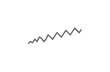
\begin{tikzpicture}[x=0.08em, y=0.08em, line width=0.4pt]
                \draw[FooterGray] (0,3) -- (1,4) -- (2,3.5) -- (3,5) -- (4,4) -- (5,6) -- (6,5.5) -- (7,4) -- (8,5) -- (9,7) -- (10,6) -- (11,5) -- (12,6.5) -- (13,8) -- (14,7) -- (15,6) -- (16,7.5) -- (17,9) -- (18,8) -- (19,7) -- (20,8.5) -- (21,10) -- (22,9) -- (23,8) -- (24,9.5);
            \end{tikzpicture}%
        }%
        \hskip0.5cm%
    }%
    \vskip6pt%
}

%=============================================================================
% PACHETE
%=============================================================================
\usepackage[utf8]{inputenc}
\usepackage[T1]{fontenc}
\usepackage{amsmath, amssymb, amsthm}
\usepackage{mathtools}
\usepackage{bm}
\usepackage{tikz}
\usetikzlibrary{arrows.meta, positioning, shapes, calc, decorations.pathreplacing, shadings}
\usepackage{booktabs}
\usepackage{multirow}
\usepackage{array}
\usepackage{graphicx}
\usepackage{hyperref}
\usepackage{colortbl}
\hypersetup{colorlinks=true, linkcolor=MainBlue, urlcolor=MainBlue}
\graphicspath{{../../logos/}{../../charts/}}
\hfuzz=2pt  % Suppress tiny overfull warnings (<2pt)

%=============================================================================
% COMANDA QUANTLET
%=============================================================================
\newcommand{\quantlet}[2]{%
    \hfill\href{#2}{%
        \raisebox{-0.15em}{\includegraphics[height=0.7em]{ql_logo.png}}%
        \textcolor{MainBlue}{\tiny\ #1}%
    }%
}

% Comandă pentru Quantlet sign sub grafice/tabele (format vechi, pentru compatibilitate)
\newcommand{\quantletsign}[1]{%
    \vspace{-2mm}%
    \hfill{\scriptsize\textcolor{MediumGray}{\faCode\ Quantlet: #1}}%
}

%=============================================================================
% MEDII PENTRU TEOREME
%=============================================================================
\theoremstyle{definition}
\setbeamertemplate{theorems}[numbered]
\newtheorem{defn}{Definiție}
\newtheorem{thm}{Teoremă}
\newtheorem{prop}{Propoziție}
\newtheorem{rmk}{Observație}

%=============================================================================
% COMENZI PERSONALIZATE
%=============================================================================
\newcommand{\E}{\mathbb{E}}
\newcommand{\Var}{\text{Var}}
\newcommand{\Cov}{\text{Cov}}
\newcommand{\Corr}{\text{Corr}}
\newcommand{\R}{\mathbb{R}}
\newcommand{\N}{\mathbb{N}}
\newcommand{\Z}{\mathbb{Z}}
\newcommand{\B}{\mathbf{B}}
\newcommand{\imark}{\textcolor{MainBlue}{\textbullet}}

%=============================================================================
% PAGINĂ TITLU PERSONALIZATĂ
%=============================================================================
\defbeamertemplate*{title page}{hybrid}[1][]
{
    \vspace{0.2cm}
    % Logos row - top header (with clickable links)
    \begin{center}
        \href{https://www.ase.ro}{\includegraphics[height=1.0cm]{ase_logo.png}}\hspace{0.3cm}%
        \href{https://theida.net}{\includegraphics[height=1.0cm]{ida_logo.png}}\hspace{0.3cm}%
        \href{https://blockchain-research-center.com}{\includegraphics[height=1.0cm]{brc_logo.png}}\hspace{0.3cm}%
        \href{https://www.ai4efin.ase.ro}{\includegraphics[height=1.0cm]{ai4efin_logo.png}}\hspace{0.3cm}%
        \href{https://ipe.ro/new}{\includegraphics[height=1.0cm]{acad_logo.png}}\hspace{0.3cm}%
        \href{https://www.digital-finance-msca.com}{\includegraphics[height=1.0cm]{msca_logo.png}}%
    \end{center}

    \vspace{0.6cm}

    % Main title with Q logos on sides (with clickable links)
    \begin{center}
        \begin{minipage}{0.1\textwidth}
            \centering
            \href{https://quantlet.com}{\includegraphics[height=1.1cm]{ql_logo.png}}
        \end{minipage}%
        \begin{minipage}{0.78\textwidth}
            \centering
            {\LARGE\bfseries\usebeamercolor[fg]{title}\inserttitle}

            \vspace{0.3cm}

            {\usebeamerfont{subtitle}\usebeamercolor[fg]{title}\insertsubtitle}
        \end{minipage}%
        \begin{minipage}{0.1\textwidth}
            \centering
            \href{https://quantinar.com}{\includegraphics[height=1.1cm]{qr_logo.png}}
        \end{minipage}
    \end{center}

    \vspace{0.6cm}

    % Authors (left aligned)
    \hspace{0.5cm}{\usebeamerfont{author}\insertauthor}

    \vspace{0.3cm}

    % Institute/Affiliations (left aligned)
    \hspace{0.5cm}\begin{minipage}[t]{0.9\textwidth}
        \raggedright\small\insertinstitute
    \end{minipage}
}

%=============================================================================
% INFORMAȚII TITLU
%=============================================================================
\title[Analiza Seriilor de Timp]{Analiza și Prognoza seriilor de timp}
\subtitle{Capitolul 3: Modele ARIMA pentru Date Nestaționare}
\author[D.T. Pele]{Daniel Traian PELE}
\institute{Academia de Studii Economice din București\\
IDA Institute Digital Assets\\
Blockchain Research Center\\
AI4EFin Artificial Intelligence for Energy Finance\\
Academia Română, Institutul de Prognoză Economică\\
MSCA Digital Finance}
\date{}

\begin{document}

% Title page (no header/footer)
{
\setbeamertemplate{headline}{}
\setbeamertemplate{footline}{}
\begin{frame}
    \titlepage
\end{frame}
}

%=============================================================================
% CUPRINS
%=============================================================================
\begin{frame}{Structura cursului}
    \vspace{-0.3cm}
    {\small
    \begin{columns}[T]
        \begin{column}{0.48\textwidth}
            \tableofcontents[sections={1-6}, hideallsubsections]
        \end{column}
        \begin{column}{0.48\textwidth}
            \tableofcontents[sections={7-11}, hideallsubsections]
        \end{column}
    \end{columns}
    }
\end{frame}

%=============================================================================
% MOTIVAȚIE
%=============================================================================
\section{Motivație}

\begin{frame}{De ce ARIMA? Datele nestaționare sunt pretutindeni}
    \vspace{-0.3cm}
    \begin{center}
        \includegraphics[width=0.88\textwidth, height=0.58\textheight, keepaspectratio]{ch3_motivation_nonstationary.pdf}
    \end{center}
    \vspace{-0.2cm}
    {\footnotesize
    \begin{itemize}\setlength{\itemsep}{0pt}
        \item Prețurile acțiunilor, PIB, cursurile de schimb prezintă \textbf{trenduri} sau \textbf{comportament rătăcitor}
        \item Media din eșantion (linia roșie) este lipsită de sens pentru un mers aleatoriu ($\bar{x} = \frac{1}{n}\sum_{i=1}^n x_i$)
        \item Modelele ARMA standard \textbf{nu pot} gestiona aceste serii direct
    \end{itemize}
    }\quantlet{TSA\_ch3\_motivation\_nonstationary}{https://github.com/QuantLet/TSA/tree/main/TSA_ch3_motivation_nonstationary}
\end{frame}

\begin{frame}{Aplicații practice}
    \begin{columns}[T]
        \column{0.35\textwidth}
        \begin{alertblock}{Provocarea}
            \begin{itemize}\setlength{\itemsep}{0pt}
                \item Prețuri de acțiuni: mers aleatoriu în logaritmi
                \item Cursuri de schimb: mers aleatoriu
                \item Rate ale dobânzii: foarte persistente
                    \begin{itemize}\setlength{\itemsep}{0pt}
                        \item Aproape de rădăcină unitate
                    \end{itemize}
            \end{itemize}
        \end{alertblock}
        \column{0.63\textwidth}
        \vspace{-0.3cm}
        \begin{center}
            \includegraphics[width=\textwidth, height=0.78\textheight, keepaspectratio]{ch3_motivation_realworld.pdf}
        \end{center}
    \end{columns}
    \quantlet{TSA\_ch3\_motivation\_realworld}{https://github.com/QuantLet/TSA/tree/main/TSA_ch3_motivation_realworld}
\end{frame}

\begin{frame}{Soluția: diferențierea}
    \vspace{-0.3cm}
    \begin{center}
        \includegraphics[width=0.88\textwidth, height=0.62\textheight, keepaspectratio]{ch3_motivation_differencing.pdf}
    \end{center}
    \vspace{-0.2cm}
    {\footnotesize
    \begin{exampleblock}{Observație Cheie}
        \textbf{Diferențierea} transformă o serie nestaționară într-una staționară:
        $\Delta Y_t = Y_t - Y_{t-1}$. ACF se schimbă de la descreștere lentă la descreștere rapidă!
    \end{exampleblock}
    }\quantlet{TSA\_ch3\_motivation\_differencing}{https://github.com/QuantLet/TSA/tree/main/TSA_ch3_motivation_differencing}
\end{frame}

\begin{frame}{Ce vom învăța astăzi}
    \begin{block}{Concepte Fundamentale}
        \begin{enumerate}
            \item \textbf{Nestaționaritatea}: De ce contează și cum o detectăm
            \item \textbf{Teste de rădăcină unitate}: Testele ADF, PP, KPSS
            \item \textbf{Diferențierea}: Transformarea cheie
            \item \textbf{Modele ARIMA}: Combinarea diferențierii cu ARMA
            \item \textbf{Metodologia Box-Jenkins}: Identificare $\to$ Estimare $\to$ Validare
        \end{enumerate}
    \end{block}

    \vspace{0.2cm}

    \begin{exampleblock}{La sfârșitul acestui curs}
        Veți fi capabili să modelați și să prognozați serii de timp nestaționare precum prețurile acțiunilor, PIB și cursurile de schimb folosind modele ARIMA.
    \end{exampleblock}
\end{frame}

%=============================================================================
% SECȚIUNEA 1: NESTAȚIONARITATEA
%=============================================================================
\section{Nestaționaritatea în seriile de timp}

\begin{frame}{De ce contează nestaționaritatea}
    {\small
    \begin{alertblock}{Problema}
        Multe serii de timp economice și financiare sunt \textbf{nestaționare}:
        \begin{itemize}\setlength{\itemsep}{0pt}
            \item PIB, prețuri de acțiuni, cursuri de schimb, indici de inflație
            \item Prezintă trenduri, medii în schimbare sau varianță în creștere
        \end{itemize}
    \end{alertblock}

    \vspace{0.1cm}

    \begin{block}{Consecințele Nestaționarității}
        \begin{itemize}\setlength{\itemsep}{0pt}
            \item Modelele ARMA standard presupun staționaritate
            \item Regresia OLS cu date nestaționare duce la \textbf{regresie falsă}
            \item Momentele din eșantion (medie, varianță, ACF) nu sunt estimatori consistenți
            \item Inferența statistică devine invalidă
        \end{itemize}
    \end{block}
    }
\end{frame}

\begin{frame}{Exemplu: PIB real SUA}
    \begin{columns}[T]
        \column{0.35\textwidth}
        \begin{block}{Observații}
            \begin{itemize}\setlength{\itemsep}{0pt}
                \item \textbf{Trend} ascendent clar -- media nu este constantă
                \item Exemplu clasic de serie \textbf{nestaționară}
                \item Nu putem aplica modele ARMA direct
            \end{itemize}
        \end{block}
        \column{0.63\textwidth}
        \vspace{-0.3cm}
        \begin{center}
            \includegraphics[width=\textwidth, height=0.78\textheight, keepaspectratio]{ch3_gdp_levels.pdf}
        \end{center}
    \end{columns}
    \quantlet{TSA\_ch3\_gdp\_levels}{https://github.com/QuantLet/TSA/tree/main/TSA_ch3_gdp_levels}
\end{frame}

\begin{frame}{Tipuri de nestaționaritate}
    \begin{columns}[T]
        \begin{column}{0.48\textwidth}
            \begin{block}{Trend determinist}
                $$Y_t = \alpha + \beta t + \varepsilon_t$$
                \begin{itemize}
                    \item Trendul este o funcție deterministă de timp
                    \item Poate fi eliminat prin \textbf{regresie}
                    \item Șocurile au efecte temporare
                \end{itemize}
            \end{block}
        \end{column}
        \begin{column}{0.48\textwidth}
            \begin{block}{Trend stochastic (Rădăcină Unitate)}
                $$Y_t = Y_{t-1} + \varepsilon_t$$
                \begin{itemize}
                    \item Proces de mers aleatoriu
                    \item Trebuie eliminat prin \textbf{diferențiere}
                    \item Șocurile au efecte permanente
                \end{itemize}
            \end{block}
        \end{column}
    \end{columns}

    \vspace{0.5cm}

    \begin{alertblock}{Distincție Cheie}
        Identificarea corectă este crucială: eliminarea trendului prin regresie pentru un proces cu rădăcină unitară sau diferențierea unui proces staționar în trend duc ambele la specificare greșită!
    \end{alertblock}
\end{frame}

\begin{frame}{Vizualizarea diferenței}
    \begin{columns}[T]
        \column{0.35\textwidth}
        \begin{block}{Observații}
            \begin{itemize}\setlength{\itemsep}{0pt}
                \item \textbf{Stânga}: Trend determinist
                    \begin{itemize}\setlength{\itemsep}{0pt}
                        \item Abaterile de la trend sunt temporare
                    \end{itemize}
                \item \textbf{Dreapta}: Trend stochastic
                    \begin{itemize}\setlength{\itemsep}{0pt}
                        \item Șocurile se acumulează permanent
                    \end{itemize}
                \item Ambele arată similar, dar necesită tratamente \textbf{diferite}!
            \end{itemize}
        \end{block}
        \column{0.63\textwidth}
        \vspace{-0.3cm}
        \begin{center}
            \includegraphics[width=\textwidth, height=0.78\textheight, keepaspectratio]{ch3_trend_comparison.pdf}
        \end{center}
    \end{columns}
    \quantlet{TSA\_ch3\_trend\_comparison}{https://github.com/QuantLet/TSA/tree/main/TSA_ch3_trend_comparison}
\end{frame}

\begin{frame}{Procesul de mers aleatoriu}
    {\small
    \begin{defn}[Mers aleatoriu]
        Un \textbf{mers aleatoriu} este definit ca:
        $$Y_t = Y_{t-1} + \varepsilon_t, \quad \varepsilon_t \sim WN(0, \sigma^2)$$
        Cu condiția inițială $Y_0 = 0$, avem: $Y_t = \sum_{i=1}^{t} \varepsilon_i$
    \end{defn}

    \vspace{0.1cm}

    \begin{block}{Proprietățile Mersului Aleatoriu}
        \begin{itemize}\setlength{\itemsep}{0pt}
            \item $\E[Y_t] = 0$ (medie constantă)
            \item $\Var(Y_t) = t\sigma^2$ (varianța crește în timp!)
            \item $\Cov(Y_t, Y_{t-k}) = (t-k)\sigma^2$ pentru $k \leq t$
            \item ACF: $\rho_k = \sqrt{\frac{t-k}{t}} \to 1$ când $t \to \infty$
        \end{itemize}
    \end{block}
    }
\end{frame}

\begin{frame}{Mers aleatoriu: ilustrație vizuală}
    \begin{columns}[T]
        \column{0.35\textwidth}
        \begin{alertblock}{Proprietăți cheie}
            \begin{itemize}\setlength{\itemsep}{0pt}
                \item \textbf{Stânga}: Traiectorii rătăcesc imprevizibil, fără revenire la medie
                \item \textbf{Dreapta}: $\Var(Y_t) = t\sigma^2$ crește liniar
                    \begin{itemize}\setlength{\itemsep}{0pt}
                        \item Caracteristica definitorie a nestaționarității
                    \end{itemize}
            \end{itemize}
        \end{alertblock}
        \column{0.63\textwidth}
        \vspace{-0.3cm}
        \begin{center}
            \includegraphics[width=\textwidth, height=0.78\textheight, keepaspectratio]{ch3_def_random_walk.pdf}
        \end{center}
    \end{columns}
    \quantlet{TSA\_ch3\_def\_random\_walk}{https://github.com/QuantLet/TSA/tree/main/TSA_ch3_def_random_walk}
\end{frame}

\begin{frame}{Demonstrație: varianța mersului aleatoriu}
    \textbf{Afirmație:} Pentru $Y_t = Y_{t-1} + \varepsilon_t$ cu $Y_0 = 0$: $\Var(Y_t) = t\sigma^2$

    \vspace{0.1cm}
    \textbf{Demonstrație:} Prin substituție recursivă:
    $$Y_t = Y_{t-1} + \varepsilon_t = Y_{t-2} + \varepsilon_{t-1} + \varepsilon_t = \cdots = \sum_{i=1}^{t} \varepsilon_i$$

    Luând varianța:
    $$\Var(Y_t) = \Var\left(\sum_{i=1}^{t} \varepsilon_i\right) = \sum_{i=1}^{t} \Var(\varepsilon_i) + 2\sum_{i<j} \Cov(\varepsilon_i, \varepsilon_j)$$
    \vspace{-2mm}

    Deoarece $\varepsilon_t$ sunt independente (zgomot alb), toate covarianțele sunt zero:
    $\Var(Y_t) = \sum_{i=1}^{t} \sigma^2 = \boxed{t\sigma^2}$

    \begin{alertblock}{Nestaționaritate}
        Varianța depinde de $t$ $\Rightarrow$ încalcă cerința staționarității ($\Var(Y_t) = \gamma(0)$ constant).
    \end{alertblock}
\end{frame}

\begin{frame}{Demonstrație: autocovarianța mersului aleatoriu}
    \textbf{Afirmație:} $\Cov(Y_t, Y_{t-k}) = (t-k)\sigma^2$ pentru $k \leq t$

    \vspace{0.2cm}
    \textbf{Demonstrație:} Folosind $Y_t = \sum_{i=1}^{t} \varepsilon_i$ și $Y_{t-k} = \sum_{i=1}^{t-k} \varepsilon_i$:
    \begin{align*}
    \Cov(Y_t, Y_{t-k}) &= \Cov\left(\sum_{i=1}^{t} \varepsilon_i, \sum_{j=1}^{t-k} \varepsilon_j\right) \\
    &= \sum_{i=1}^{t}\sum_{j=1}^{t-k} \Cov(\varepsilon_i, \varepsilon_j) = \sum_{i=1}^{t-k} \Var(\varepsilon_i) = \boxed{(t-k)\sigma^2}
    \end{align*}

    Doar termenii cu $i = j$ supraviețuiesc (când $i \leq t-k$).

    \vspace{0.1cm}
    \textbf{ACF:}
    $$\rho(k) = \frac{\Cov(Y_t, Y_{t-k})}{\sqrt{\Var(Y_t)\Var(Y_{t-k})}} = \frac{(t-k)\sigma^2}{\sqrt{t\sigma^2 \cdot (t-k)\sigma^2}} = \sqrt{\frac{t-k}{t}}$$
\end{frame}

\begin{frame}{Mers aleatoriu cu drift}
    {\small
    \begin{defn}[Mers aleatoriu cu drift]
        Un mers aleatoriu cu drift include un termen constant:
        $$Y_t = \mu + Y_{t-1} + \varepsilon_t$$
        Echivalent: $Y_t = Y_0 + \mu t + \sum_{i=1}^{t} \varepsilon_i$
    \end{defn}

    \vspace{0.1cm}

    \begin{block}{Proprietăți}
        \begin{itemize}\setlength{\itemsep}{0pt}
            \item $\E[Y_t] = Y_0 + \mu t$ (media crește liniar)
            \item $\Var(Y_t) = t\sigma^2$ (varianța tot crește)
            \item Drift-ul $\mu$ creează un trend ascendent sau descendent
            \item Tot nestaționar în ciuda faptului că are un ``trend''
        \end{itemize}
    \end{block}
    }
\end{frame}

\begin{frame}{Mers aleatoriu cu drift: ilustrație vizuală}
    \begin{columns}[T]
        \column{0.35\textwidth}
        \begin{exampleblock}{Comparație}
            \begin{itemize}\setlength{\itemsep}{0pt}
                \item \textbf{Fără drift} (albastru): rătăcește în jurul lui zero
                \item \textbf{Cu drift} $\mu > 0$ (roșu): trend ascendent sistematic
                \item Ambele sunt nestaționare
                    \begin{itemize}\setlength{\itemsep}{0pt}
                        \item Drift-ul adaugă trend determinist la rătăcirea stocastică
                    \end{itemize}
            \end{itemize}
        \end{exampleblock}
        \column{0.63\textwidth}
        \vspace{-0.3cm}
        \begin{center}
            \includegraphics[width=\textwidth, height=0.78\textheight, keepaspectratio]{ch3_def_random_walk_drift.pdf}
        \end{center}
    \end{columns}
    \quantlet{TSA\_ch3\_def\_random\_walk\_drift}{https://github.com/QuantLet/TSA/tree/main/TSA_ch3_def_random_walk_drift}
\end{frame}

\begin{frame}{Simularea mersurilor aleatorii}
    \begin{columns}[T]
        \column{0.35\textwidth}
        \begin{block}{Observații}
            \begin{itemize}\setlength{\itemsep}{0pt}
                \item \textbf{Stânga}: Mersuri aleatorii pure -- fără drift, rătăcesc imprevizibil
                \item \textbf{Dreapta}: Cu drift -- trend ascendent în medie
                \item Fiecare traiectorie este unică
                    \begin{itemize}\setlength{\itemsep}{0pt}
                        \item Incertitudinea crește în timp
                    \end{itemize}
            \end{itemize}
        \end{block}
        \column{0.63\textwidth}
        \vspace{-0.3cm}
        \begin{center}
            \includegraphics[width=\textwidth, height=0.78\textheight, keepaspectratio]{ch3_random_walk.pdf}
        \end{center}
    \end{columns}
    \quantlet{TSA\_ch3\_random\_walk}{https://github.com/QuantLet/TSA/tree/main/TSA_ch3_random_walk}
\end{frame}

\begin{frame}{Creșterea varianței: de ce mersurile aleatorii sunt nestaționare}
    \begin{columns}[T]
        \column{0.35\textwidth}
        \begin{block}{Observații}
            \begin{itemize}\setlength{\itemsep}{0pt}
                \item \textbf{Stânga}: Evantaiul de traiectorii arată incertitudinea crescând
                \item \textbf{Dreapta}: Varianța crește liniar: $\Var(Y_t) = t\sigma^2$
                \item Aceasta violează staționaritatea
                    \begin{itemize}\setlength{\itemsep}{0pt}
                        \item Varianța ar trebui să fie constantă
                    \end{itemize}
            \end{itemize}
        \end{block}
        \column{0.63\textwidth}
        \vspace{-0.3cm}
        \begin{center}
            \includegraphics[width=\textwidth, height=0.78\textheight, keepaspectratio]{ch3_variance_growth.pdf}
        \end{center}
    \end{columns}
    \quantlet{TSA\_ch3\_variance\_growth}{https://github.com/QuantLet/TSA/tree/main/TSA_ch3_variance_growth}
\end{frame}

\begin{frame}{Procese integrate}
    {\small
    \begin{defn}[Proces Integrat de Ordin $d$]
        O serie de timp $\{Y_t\}$ este \textbf{integrată de ordin $d$}, scrisă $Y_t \sim I(d)$, dacă:
        \begin{itemize}\setlength{\itemsep}{0pt}
            \item $Y_t$ este nestaționară
            \item $(1-L)^d Y_t = \Delta^d Y_t$ este staționară
            \item $(1-L)^{d-1} Y_t$ este încă nestaționară
        \end{itemize}
    \end{defn}

    \vspace{0.1cm}

    \begin{exampleblock}{Cazuri Comune}
        \begin{itemize}\setlength{\itemsep}{0pt}
            \item $I(0)$: Proces staționar (de ex., ARMA)
            \item $I(1)$: Prima diferență este staționară (cel mai frecvent pentru date economice)
            \item $I(2)$: A doua diferență este staționară (mai rar)
        \end{itemize}
    \end{exampleblock}
    }
\end{frame}

\begin{frame}{Proces integrat: ilustrație vizuală}
    \begin{columns}[T]
        \column{0.35\textwidth}
        \begin{block}{Ordinul de integrare}
            \begin{itemize}\setlength{\itemsep}{0pt}
                \item $I(0)$: Staționar --- nicio diferențiere necesară
                \item $I(1)$: O diferență necesară (mers aleatoriu)
                \item $I(2)$: Două diferențe necesare
                \item Majoritatea seriilor economice sunt $I(0)$ sau $I(1)$
            \end{itemize}
        \end{block}
        \column{0.63\textwidth}
        \vspace{-0.3cm}
        \begin{center}
            \includegraphics[width=\textwidth, height=0.78\textheight, keepaspectratio]{ch3_def_integrated.pdf}
        \end{center}
    \end{columns}
    \quantlet{TSA\_ch3\_def\_integrated}{https://github.com/QuantLet/TSA/tree/main/TSA_ch3_def_integrated}
\end{frame}

%=============================================================================
% SECȚIUNEA 2: DIFERENȚIEREA
%=============================================================================
\section{Diferențierea și Operatorul diferență}

\begin{frame}{Operatorul diferență}
    {\small
    \begin{defn}[Prima Diferență]
        \textbf{Operatorul primei diferențe} $\Delta$ este definit ca:
        $\Delta Y_t = Y_t - Y_{t-1} = (1-L)Y_t$, unde $L$ este operatorul lag ($LY_t = Y_{t-1}$).
    \end{defn}

    \vspace{0.1cm}

    \begin{block}{Diferențe de Ordin Superior}
        \begin{itemize}\setlength{\itemsep}{0pt}
            \item A două diferență: $\Delta^2 Y_t = \Delta(\Delta Y_t) = (1-L)^2 Y_t$
            \item $\Delta^2 Y_t = Y_t - 2Y_{t-1} + Y_{t-2}$
            \item Diferența de ordin $d$: $\Delta^d Y_t = (1-L)^d Y_t$
        \end{itemize}
    \end{block}

    \vspace{0.1cm}

    \begin{alertblock}{Rezultat Cheie}
        Dacă $Y_t \sim I(d)$, atunci $\Delta^d Y_t \sim I(0)$ (staționar).
    \end{alertblock}
    }
\end{frame}

\begin{frame}{Prima diferență: ilustrație vizuală}
    \begin{center}
        \includegraphics[width=0.95\textwidth]{ch3_def_difference.pdf}
    \end{center}
    \vspace{-0.2cm}
    \small Stânga: serie nestaționară. Dreapta: după prima diferență, seria devine staționară.
    \quantlet{TSA\_ch3\_def\_difference}{https://github.com/QuantLet/TSA/tree/main/TSA_ch3_def_difference}
\end{frame}

\begin{frame}{Exemplu: diferențierea unui mers aleatoriu}
    {\small
    \begin{exampleblock}{Mers aleatoriu la Zgomot Alb}
        Fie $Y_t = Y_{t-1} + \varepsilon_t$ (mers aleatoriu). Luând prima diferență:
        $$\Delta Y_t = Y_t - Y_{t-1} = \varepsilon_t$$
        Prima diferență este zgomot alb -- un proces staționar!
    \end{exampleblock}

    \vspace{0.1cm}

    \begin{block}{Interpretare}
        \begin{itemize}\setlength{\itemsep}{0pt}
            \item Un mers aleatoriu este $I(1)$
            \item O diferență îl transformă în $I(0)$
            \item ``Schimbările'' într-un mers aleatoriu sunt staționare
        \end{itemize}
    \end{block}
    }
\end{frame}

\begin{frame}{Demonstrație: diferențierea induce staționaritatea}
    \textbf{Afirmație:} Dacă $Y_t \sim I(1)$, atunci $\Delta Y_t = Y_t - Y_{t-1}$ este staționar.

    \vspace{0.15cm}
    \textbf{Demonstrație pentru Mers aleatoriu cu drift:} $Y_t = \mu + Y_{t-1} + \varepsilon_t$

    Prima diferență este:
    $$\Delta Y_t = Y_t - Y_{t-1} = \mu + \varepsilon_t$$

    Verificăm condițiile de staționaritate:
    \begin{enumerate}
        \item \textbf{Media:} $\E[\Delta Y_t] = \mu$ (constantă, nu depinde de $t$) \checkmark
        \item \textbf{Varianța:} $\Var(\Delta Y_t) = \Var(\varepsilon_t) = \sigma^2$ (constantă) \checkmark
        \item \textbf{Autocovarianța:} $\Cov(\Delta Y_t, \Delta Y_{t-k}) = \Cov(\varepsilon_t, \varepsilon_{t-k}) = 0$ pentru $k \neq 0$ \checkmark
    \end{enumerate}

    \begin{exampleblock}{Principiu General}
        Diferențierea elimină ``memoria'' care face varianța să se acumuleze. Pentru procese $I(d)$, sunt necesare $d$ diferențe.
    \end{exampleblock}
\end{frame}

\begin{frame}{ACF: detectarea nestaționarității}
    \vspace{-0.3cm}
    \begin{center}
        \includegraphics[width=0.92\textwidth, height=0.68\textheight, keepaspectratio]{ch3_acf_nonstationary.pdf}
    \end{center}
    \vspace{-0.2cm}
    {\footnotesize
    \begin{itemize}
        \item \textbf{Sus}: ACF mers aleatoriu scade foarte lent $\Rightarrow$ rădăcină unitate
        \item \textbf{Jos}: După diferențiere, ACF se întrerupe $\Rightarrow$ staționar
    \end{itemize}
    }\quantlet{TSA\_ch3\_acf\_nonstationary}{https://github.com/QuantLet/TSA/tree/main/TSA_ch3_acf_nonstationary}
\end{frame}

\begin{frame}{Diferențierea în practică: exemplul PIB}
    \vspace{-0.3cm}
    \begin{center}
        \includegraphics[width=0.92\textwidth, height=0.65\textheight, keepaspectratio]{ch3_differencing.pdf}
    \end{center}
    \vspace{-0.2cm}
    {\footnotesize
    \begin{itemize}
        \item \textbf{Stânga}: PIB în niveluri -- trend ascendent clar (nestaționar)
        \item \textbf{Dreapta}: Rata de creștere PIB (diferența logaritmică) -- fluctuează în jurul mediei (staționar)
        \item Diferențierea elimină trendul și obține staționaritate
    \end{itemize}
    }\quantlet{TSA\_ch3\_differencing}{https://github.com/QuantLet/TSA/tree/main/TSA_ch3_differencing}
\end{frame}

\begin{frame}{Supra-diferențierea}
    {\small
    \begin{alertblock}{Avertisment: Supra-diferențierea}
        Diferențierea mai mult decât este necesar introduce probleme:
        \begin{itemize}\setlength{\itemsep}{0pt}
            \item Creează autocorelație negativă artificială
            \item Inflează varianța
            \item Pierde informație
        \end{itemize}
    \end{alertblock}

    \vspace{0.1cm}

    \begin{exampleblock}{Exemplu}
        Dacă $Y_t \sim I(1)$, atunci $\Delta Y_t \sim I(0)$. Dar dacă diferențiem din nou:
        $$\Delta^2 Y_t = \Delta Y_t - \Delta Y_{t-1} = \varepsilon_t - \varepsilon_{t-1}$$
        Acesta este un MA(1) cu $\theta_1 = -1$ (la granița non-invertibilității)!
    \end{exampleblock}
    }
\end{frame}

%=============================================================================
% SECȚIUNEA 3: MODELE ARIMA
%=============================================================================
\section{Modele ARIMA(p,d,q)}

\begin{frame}{Definiția ARIMA}
    {\small
    \begin{defn}[ARIMA(p,d,q)]
        O serie de timp $\{Y_t\}$ urmează un proces \textbf{ARIMA(p,d,q)} dacă:
        $$\phi(L)(1-L)^d Y_t = c + \theta(L)\varepsilon_t$$
        unde:
        \begin{itemize}\setlength{\itemsep}{0pt}
            \item $\phi(L) = 1 - \phi_1 L - \phi_2 L^2 - \cdots - \phi_p L^p$ (polinomul AR)
            \item $\theta(L) = 1 + \theta_1 L + \theta_2 L^2 + \cdots + \theta_q L^q$ (polinomul MA)
            \item $d$ este ordinul de integrare (numărul de diferențe)
            \item $\varepsilon_t \sim WN(0, \sigma^2)$
        \end{itemize}
    \end{defn}
    }
\end{frame}

\begin{frame}{ARIMA: ilustrație vizuală}
    \begin{columns}[T]
        \column{0.35\textwidth}
        \begin{exampleblock}{Interpretare}
            \begin{itemize}\setlength{\itemsep}{0pt}
                \item \textbf{Sus}: seria ARIMA originală (nestaționară)
                \item \textbf{Jos}: după diferențiere de $d$ ori
                    \begin{itemize}\setlength{\itemsep}{0pt}
                        \item ACF/PACF dezvăluie ordinele AR și MA
                    \end{itemize}
            \end{itemize}
        \end{exampleblock}
        \column{0.63\textwidth}
        \vspace{-0.3cm}
        \begin{center}
            \includegraphics[width=\textwidth, height=0.78\textheight, keepaspectratio]{ch3_def_arima.pdf}
        \end{center}
    \end{columns}
    \quantlet{TSA\_ch3\_def\_arima}{https://github.com/QuantLet/TSA/tree/main/TSA_ch3_def_arima}
\end{frame}

\begin{frame}{Componentele ARIMA}
    \begin{center}
        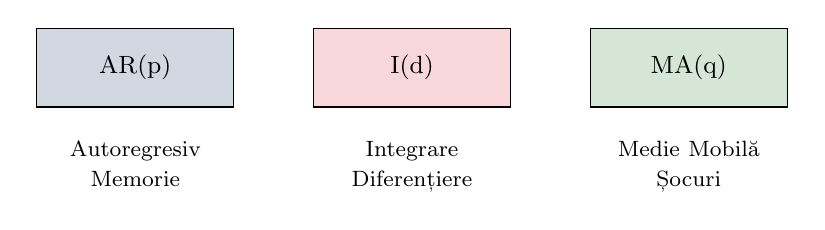
\begin{tikzpicture}[node distance=2cm, every node/.style={font=\small}]
            \node[draw, rectangle, fill=MainBlue!20, minimum width=2.5cm, minimum height=1cm] (AR) {AR(p)};
            \node[draw, rectangle, fill=Crimson!20, minimum width=2.5cm, minimum height=1cm, right=1cm of AR] (I) {I(d)};
            \node[draw, rectangle, fill=Forest!20, minimum width=2.5cm, minimum height=1cm, right=1cm of I] (MA) {MA(q)};

            \node[below=0.3cm of AR, text width=2.5cm, align=center] {\footnotesize Autoregresiv\\Memorie};
            \node[below=0.3cm of I, text width=2.5cm, align=center] {\footnotesize Integrare\\Diferențiere};
            \node[below=0.3cm of MA, text width=2.5cm, align=center] {\footnotesize Medie Mobilă\\Șocuri};
        \end{tikzpicture}
    \end{center}

    \vspace{0.2cm}

    {\small
    \begin{block}{Cazuri Speciale}
        \begin{itemize}\setlength{\itemsep}{0pt}
            \item ARIMA(p,0,q) = ARMA(p,q) -- staționar
            \item ARIMA(0,1,0) = Mers aleatoriu
            \item ARIMA(0,1,1) = IMA(1,1) -- netezire exponențială
            \item ARIMA(1,1,0) = ARI(1,1) -- AR(1) diferențiat
        \end{itemize}
    \end{block}
    }
\end{frame}

\begin{frame}{Exemplu ARIMA(1,1,0)}
    {\small
    \begin{exampleblock}{Model ARI(1,1)}
        $$\Delta Y_t = c + \phi_1 \Delta Y_{t-1} + \varepsilon_t$$
        Echivalent: $(1-\phi_1 L)(1-L)Y_t = c + \varepsilon_t$
    \end{exampleblock}

    \vspace{0.1cm}

    \begin{block}{Interpretare}
        \begin{itemize}\setlength{\itemsep}{0pt}
            \item \textbf{Schimbările} în $Y_t$ urmează un proces AR(1)
            \item Dacă $|\phi_1| < 1$, schimbările sunt staționare
            \item $Y_t$ în sine are un trend stochastic
            \item Model comun pentru multe serii de timp economice
        \end{itemize}
    \end{block}
    }
\end{frame}

\begin{frame}{Exemplu ARIMA(0,1,1)}
    {\small
    \begin{exampleblock}{Model IMA(1,1)}
        $$\Delta Y_t = c + \varepsilon_t + \theta_1 \varepsilon_{t-1}$$
        Echivalent: $(1-L)Y_t = c + (1+\theta_1 L)\varepsilon_t$
    \end{exampleblock}

    \vspace{0.1cm}

    \begin{block}{Conexiunea cu Netezirea exponențială}
        Modelul IMA(1,1) este echivalent cu \textbf{netezirea exponențială simplă}:
        $$\hat{Y}_{t+1} = \alpha Y_t + (1-\alpha)\hat{Y}_t$$
        unde $\alpha = 1 + \theta_1$ (pentru $-1 < \theta_1 < 0$).
    \end{block}
    }
\end{frame}

\begin{frame}{Rolul constantei în ARIMA}
    {\small
    \begin{block}{Termenul Constant în ARIMA(p,d,q)}
        Când $d > 0$, constanta $c$ are o interpretare diferită:
        $\phi(L)(1-L)^d Y_t = c + \theta(L)\varepsilon_t$
    \end{block}

    \vspace{0.1cm}

    \begin{alertblock}{Implicații Importante}
        \begin{itemize}\setlength{\itemsep}{0pt}
            \item Pentru $d=1$: $c$ reprezintă \textbf{drift-ul} (schimbarea medie): $\E[\Delta Y_t] = \frac{c}{1-\phi_1-\cdots-\phi_p}$
            \item Pentru $d=2$: $c$ afectează \textbf{curbura} trendului
            \item Adesea se presupune $c=0$ când $d \geq 1$
        \end{itemize}
    \end{alertblock}
    }
\end{frame}

%=============================================================================
% SECȚIUNEA 4: TESTE DE RĂDĂCINĂ UNITATE
%=============================================================================
\section{Teste de rădăcină unitate}

\begin{frame}{Testarea pentru rădăcini unitate}
    {\small
    \begin{block}{De ce Testăm?}
        Înainte de a potrivi un model ARIMA, trebuie să determinăm:
        \begin{enumerate}\setlength{\itemsep}{0pt}
            \item Este seria staționară? (Este $d=0$?)
            \item Dacă nu, câte diferențe sunt necesare? (Care este $d$?)
        \end{enumerate}
    \end{block}

    \vspace{0.1cm}

    \begin{block}{Teste comune de rădăcină unitate}
        \begin{itemize}\setlength{\itemsep}{0pt}
            \item \textbf{Dickey-Fuller (DF)} și \textbf{Augmented Dickey-Fuller (ADF)}
            \item \textbf{Phillips-Perron (PP)}
            \item \textbf{KPSS} (test de staționaritate -- ipoteză nulă inversată)
        \end{itemize}
    \end{block}
    }
\end{frame}

\begin{frame}{Testul Dickey-Fuller}
    {\small
    \begin{block}{Configurare}
        Considerăm modelul AR(1): $Y_t = \phi Y_{t-1} + \varepsilon_t$. Scădem $Y_{t-1}$:
        $\Delta Y_t = (\phi - 1)Y_{t-1} + \varepsilon_t = \gamma Y_{t-1} + \varepsilon_t$, unde $\gamma = \phi - 1$.
    \end{block}

    \vspace{0.1cm}

    \begin{block}{Ipoteze}
        \begin{itemize}\setlength{\itemsep}{0pt}
            \item $H_0$: $\gamma = 0$ (rădăcină unitate, $\phi = 1$, nestaționar)
            \item $H_1$: $\gamma < 0$ (staționar, $|\phi| < 1$)
        \end{itemize}
    \end{block}

    \vspace{0.1cm}

    \begin{alertblock}{Problemă Cheie}
        Sub $H_0$, statistică $t$ \textbf{nu} urmează o distribuție $t$ standard! Trebuie folosite valorile critice Dickey-Fuller.
    \end{alertblock}
    }
\end{frame}

\begin{frame}{Variante ale testului Dickey-Fuller}
    {\small
    \begin{block}{Trei Specificări}
        \begin{enumerate}\setlength{\itemsep}{0pt}
            \item \textbf{Fără constantă, fără trend}: $\Delta Y_t = \gamma Y_{t-1} + \varepsilon_t$
            \item \textbf{Cu constantă (drift)}: $\Delta Y_t = \alpha + \gamma Y_{t-1} + \varepsilon_t$
            \item \textbf{Cu constantă și trend}: $\Delta Y_t = \alpha + \beta t + \gamma Y_{t-1} + \varepsilon_t$
        \end{enumerate}
    \end{block}

    \vspace{0.1cm}

    \begin{alertblock}{Alegerea Specificării Corecte}
        \begin{itemize}\setlength{\itemsep}{0pt}
            \item Examinați datele: au un trend vizibil?
            \item Includerea termenilor inutili reduce puterea
            \item Excluderea termenilor necesari duce la inferență incorectă
        \end{itemize}
    \end{alertblock}
    }
\end{frame}

\begin{frame}{Testul Augmented Dickey-Fuller (ADF)}
    \vspace{-0.2cm}
    {\small
    \begin{block}{Problema cu DF Simplu}
        Dacă există dinamică AR dincolo de AR(1), reziduurile DF vor fi autocorelate.
    \end{block}

    \vspace{0.1cm}

    \begin{defn}[Testul ADF]
        Adăugați diferențe întârziate: $\Delta Y_t = \alpha + \beta t + \gamma Y_{t-1} + \sum_{j=1}^{k} \delta_j \Delta Y_{t-j} + \varepsilon_t$

        Testați $H_0: \gamma = 0$ folosind valorile critice ADF.
    \end{defn}

    \vspace{0.1cm}

    \begin{block}{Alegerea Lungimii Lag-ului $k$}
        \begin{itemize}
            \item Folosiți criterii informaționale (AIC, BIC)
            \item Începeți cu $k_{max}$, reduceți până ultimul lag este semnificativ
        \end{itemize}
    \end{block}
    }
\end{frame}

\begin{frame}{Testul ADF: ilustrație vizuală}
    \begin{center}
        \includegraphics[width=0.95\textwidth]{ch3_def_adf.pdf}
    \end{center}
    \vspace{-0.2cm}
    \small Stânga: serie staționară -- ADF respinge rădăcina unitate. Dreapta: nestaționară -- ADF nu respinge.
    \quantlet{TSA\_ch3\_def\_adf}{https://github.com/QuantLet/TSA/tree/main/TSA_ch3_def_adf}
\end{frame}

\begin{frame}{Valori critice ADF}
    \vspace{-0.2cm}
    {\small
    \begin{table}
        \centering
        \begin{tabular}{lccc}
            \toprule
            \textbf{Model} & \textbf{1\%} & \textbf{5\%} & \textbf{10\%} \\
            \midrule
            Fără constantă, fără trend & $-2.58$ & $-1.95$ & $-1.62$ \\
            Cu constantă & $-3.43$ & $-2.86$ & $-2.57$ \\
            Cu constantă și trend & $-3.96$ & $-3.41$ & $-3.13$ \\
            \bottomrule
        \end{tabular}
    \end{table}
    }
    \vspace{-0.1cm}
    \begin{block}{Regula de Decizie}
        {\small
        \begin{itemize}
            \item Statistică de test $<$ valoare critică $\Rightarrow$ Respingem $H_0$ (staționar)
            \item Statistică de test $\geq$ valoare critică $\Rightarrow$ Nu respingem (rădăcină unitate)
        \end{itemize}
        }
    \end{block}
\end{frame}

\begin{frame}{Testul Phillips-Perron (PP)}
    \vspace{-0.15cm}
    {\small
    \begin{block}{Motivație}
        Ca și ADF, testează $H_0$: Rădăcină unitate vs $H_1$: Staționar, dar folosește o \textbf{corecție non-parametrică} pentru corelația serială în loc de adăugarea diferențelor întârziate.
    \end{block}

    \begin{block}{Statistică de Test}
        Testul PP modifică statistică $t$ DF:
        $$Z_t = t_{\hat{\gamma}} \cdot \sqrt{\frac{\hat{\sigma}^2}{\hat{\lambda}^2}} - \frac{T(\hat{\lambda}^2 - \hat{\sigma}^2)(se(\hat{\gamma}))}{2\hat{\lambda}^2 \cdot s}$$
        unde $\hat{\lambda}^2$ este o estimare consistentă a varianței pe termen lung folosind Newey-West.
    \end{block}

    \begin{exampleblock}{Avantaje față de ADF}
        \begin{itemize}\setlength{\itemsep}{0pt}
            \item Robust la heteroscedasticitate și corelație serială
            \item Nu necesită selectarea lungimii lag-ului (folosește lățime de bandă)
        \end{itemize}
    \end{exampleblock}
    }
\end{frame}

\begin{frame}{Testul KPSS}
    \vspace{-0.2cm}
    {\small
    \begin{block}{Ipoteze Inversate}
        Spre deosebire de ADF: $H_0$: Staționar \quad vs \quad $H_1$: Rădăcină unitate
    \end{block}

    \vspace{0.1cm}

    \begin{block}{Procedura KPSS}
        Descompunem: $Y_t = \xi t + r_t + \varepsilon_t$ unde $r_t = r_{t-1} + u_t$.
        Testăm dacă $\Var(u_t) = 0$.
    \end{block}

    \vspace{0.1cm}

    \begin{exampleblock}{Utilizare Complementară cu ADF}
        \begin{itemize}
            \item ADF respinge, KPSS nu respinge $\Rightarrow$ Staționar
            \item ADF nu respinge, KPSS respinge $\Rightarrow$ Rădăcină unitate
            \item Ambele resping sau niciunul $\Rightarrow$ Neconcludent
        \end{itemize}
    \end{exampleblock}
    }
\end{frame}

%=============================================================================
% SECȚIUNEA 5: IDENTIFICAREA MODELULUI
%=============================================================================
\section{Identificarea modelului ARIMA}

\begin{frame}{Metodologia Box-Jenkins}
    \begin{center}
        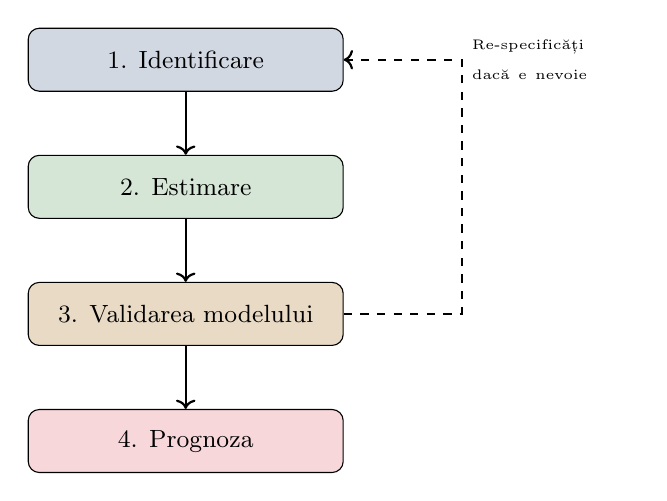
\begin{tikzpicture}[node distance=1.5cm, every node/.style={font=\small}]
            \node[draw, rectangle, rounded corners, fill=MainBlue!20, minimum width=4cm, minimum height=0.8cm] (id) {1. Identificare};
            \node[draw, rectangle, rounded corners, fill=Forest!20, minimum width=4cm, minimum height=0.8cm, below=0.8cm of id] (est) {2. Estimare};
            \node[draw, rectangle, rounded corners, fill=Amber!30, minimum width=4cm, minimum height=0.8cm, below=0.8cm of est] (diag) {3. Validarea modelului};
            \node[draw, rectangle, rounded corners, fill=Crimson!20, minimum width=4cm, minimum height=0.8cm, below=0.8cm of diag] (fore) {4. Prognoza};

            \draw[->, thick] (id) -- (est);
            \draw[->, thick] (est) -- (diag);
            \draw[->, thick] (diag) -- (fore);
            \draw[->, thick, dashed] (diag.east) -- ++(1.5,0) |- (id.east) node[midway, right, text width=2cm] {\tiny Re-specificăți dacă e nevoie};
        \end{tikzpicture}
    \end{center}
\end{frame}

\begin{frame}{Pasul 1: Determinarea lui $d$}
    {\small
    \begin{block}{Procedură}
        \begin{enumerate}\setlength{\itemsep}{0pt}
            \item Reprezentați grafic seria de timp -- căutați trenduri, varianță în schimbare
            \item Examinați ACF -- descreștere lentă sugerează nestaționaritate
            \item Aplicați teste de rădăcină unitate (ADF, KPSS)
            \item Dacă nestaționară, diferențiați și repetăți
        \end{enumerate}
    \end{block}

    \vspace{0.1cm}

    \begin{exampleblock}{Ghiduri Practice}
        \begin{itemize}\setlength{\itemsep}{0pt}
            \item Majoritatea seriilor economice: $d = 1$ este suficient
            \item Rar avem nevoie de $d > 2$
            \item Dacă ACF al $\Delta Y_t$ tot scade lent, încercați $d = 2$
            \item Atenție la supra-diferențiere (ACF cu $\rho_1 \approx -0.5$)
        \end{itemize}
    \end{exampleblock}
    }
\end{frame}

\begin{frame}{Pasul 2: Determinarea lui $p$ și $q$}
    \vspace{-0.2cm}
    {\small
    \begin{block}{După Diferențiere}
        Odată ce $W_t = \Delta^d Y_t$ este staționar, folosiți ACF/PACF pentru a identifica ARMA($p$,$q$):
    \end{block}

    \vspace{0.1cm}

    \begin{center}
        \begin{tabular}{lcc}
            \toprule
            \textbf{Model} & \textbf{ACF} & \textbf{PACF} \\
            \midrule
            AR($p$) & Scade exponențial & Se întrerupe după lag $p$ \\
            MA($q$) & Se întrerupe după lag $q$ & Scade exponențial \\
            ARMA($p$,$q$) & Scade & Scade \\
            \bottomrule
        \end{tabular}
    \end{center}

    \vspace{0.1cm}

    \begin{block}{Criterii informaționale}
        Când tiparele sunt neclare, comparați modelele folosind:
        \begin{itemize}\setlength{\itemsep}{0pt}
            \item AIC = $-2\ln(L) + 2k$; \quad BIC = $-2\ln(L) + k\ln(n)$
        \end{itemize}
        Mai mic este mai bun. BIC penalizează complexitatea mai mult.
    \end{block}
    }
\end{frame}

\begin{frame}{Algoritmi Auto-ARIMA}
    \vspace{-0.15cm}
    {\small
    \begin{block}{Selecție automată a modelului}
        Software-ul modern poate selecta automat $(p,d,q)$:
        \begin{itemize}\setlength{\itemsep}{0pt}
            \item Python: \texttt{pmdarima.auto\_arima()}
            \item R: \texttt{forecast::auto.arima()}
        \end{itemize}
    \end{block}

    \begin{block}{Cum funcționează Auto-ARIMA}
        \begin{enumerate}\setlength{\itemsep}{0pt}
            \item Folosește teste de rădăcină unitate pentru a determina $d$
            \item Potrivește modele pentru diverse combinații $(p,q)$
            \item Selectează modelul cu cel mai mic AIC/BIC
            \item Opțional folosește căutare pas cu pas pentru eficiență
        \end{enumerate}
    \end{block}

    \begin{alertblock}{Atenție}
        Selecția automată este utilă dar nu infailibilă. Verificați întotdeauna validitatea modelului!
    \end{alertblock}
    }
\end{frame}

%=============================================================================
% SECȚIUNEA 6: ESTIMARE
%=============================================================================
\section{Estimarea ARIMA}

\begin{frame}{Metode de estimare}
    {\small
    \begin{block}{Estimarea prin Maximum de Verosimilitate (MLE)}
        Abordarea standard pentru ARIMA:
        \begin{itemize}\setlength{\itemsep}{0pt}
            \item Presupune $\varepsilon_t \sim N(0, \sigma^2)$
            \item Maximizează funcția de verosimilitate
            \item Oferă estimatori consistenți, eficienți
            \item Furnizează erori standard pentru inferență
        \end{itemize}
    \end{block}

    \vspace{0.1cm}

    \begin{block}{MLE Condiționată vs Exactă}
        \begin{itemize}\setlength{\itemsep}{0pt}
            \item \textbf{MLE Condiționată}: Condiționează pe valorile inițiale
            \item \textbf{MLE Exactă}: Tratează valorile inițiale ca necunoscute
            \item Diferența diminuează pe măsură ce dimensiunea eșantionului crește
        \end{itemize}
    \end{block}
    }
\end{frame}

\begin{frame}{Log-verosimilitatea condiționată}
    \vspace{-0.2cm}
    {\footnotesize
    \begin{block}{Funcția de log-verosimilitate gaussiană}
        Pentru ARIMA$(p,d,q)$ cu $\varepsilon_t \sim N(0, \sigma^2)$:
        $\ell(\boldsymbol{\theta}, \sigma^2) = -\frac{T}{2}\ln(2\pi) - \frac{T}{2}\ln(\sigma^2) - \frac{1}{2\sigma^2}\sum_{t=1}^{T} e_t^2(\boldsymbol{\theta})$
        unde $e_t(\boldsymbol{\theta}) = X_t - \hat{X}_{t|t-1}$ sunt \textbf{erorile de predicție la un pas}, iar $\boldsymbol{\theta} = (\phi_1, \ldots, \phi_p, \theta_1, \ldots, \theta_q, c)$.
    \end{block}

    \begin{exampleblock}{Exemplu: ARIMA(1,1,1)}
        Erorile de predicție se calculează recursiv:
        $e_t = \Delta X_t - \phi_1 \Delta X_{t-1} - \theta_1 e_{t-1} - c$
        MLE condiționată: fixează $e_0 = 0$, calculează $e_1, e_2, \ldots, e_T$, maximizează $\ell$.
    \end{exampleblock}

    \begin{alertblock}{Estimarea lui $\sigma^2$}
        La parametrii optimi $\hat{\boldsymbol{\theta}}$: \quad $\hat{\sigma}^2 = \frac{1}{T}\sum_{t=1}^{T} e_t^2(\hat{\boldsymbol{\theta}})$
    \end{alertblock}
    }
\end{frame}

\begin{frame}{Restricții asupra parametrilor}
    {\small
    \begin{alertblock}{Staționaritate și invertibilitate}
        Modelul ARIMA estimat ar trebui să satisfacă:
        \begin{itemize}\setlength{\itemsep}{0pt}
            \item \textbf{Staționaritate AR}: Rădăcinile lui $\phi(z) = 0$ în afara cercului unitate
            \item \textbf{Invertibilitate MA}: Rădăcinile lui $\theta(z) = 0$ în afara cercului unitate
        \end{itemize}
    \end{alertblock}

    \vspace{0.1cm}

    \begin{block}{Verificare în Practică}
        Majoritatea software-ului raportează:
        \begin{itemize}\setlength{\itemsep}{0pt}
            \item Coeficienți estimați cu erori standard
            \item Rădăcinile polinoamelor AR și MA
            \item Avertisment dacă este detectată aproape-rădăcină-unitate
        \end{itemize}
    \end{block}
    }
\end{frame}

%=============================================================================
% SECȚIUNEA 7: DIAGNOSTICARE
%=============================================================================
\section{Diagnosticul modelului}

\begin{frame}{Diagnosticul modelului ARIMA}
    {\small
    \begin{block}{Verificări esențiale (aceleași ca pentru ARMA, cf.\ Cap.\ 2)}
        Dacă modelul este corect, reziduurile $\hat{\varepsilon}_t$ trebuie să fie zgomot alb:
        \begin{enumerate}\setlength{\itemsep}{0pt}
            \item \textbf{ACF/PACF rezidual}: fără vârfuri semnificative
            \item \textbf{Testul Ljung-Box}: p-value $> 0.05$ $\Rightarrow$ fără autocorelare
            \item \textbf{Graficul Q-Q}: verificarea normalității
            \item \textbf{Heteroscedasticitate}: varianță constantă a reziduurilor
        \end{enumerate}
    \end{block}

    \vspace{0.1cm}

    \begin{alertblock}{Aspecte specifice ARIMA}
        \begin{itemize}\setlength{\itemsep}{0pt}
            \item Testul Ljung-Box: alegeți $m \approx \ln(n)$ sau $m = 10$ (trimestrial), $m = 20$ (lunar)
            \item Grade de libertate: $\chi^2(m-p-q)$, ajustate pentru $p$ și $q$ estimați
            \item Dacă testul eșuează: adăugați termeni AR/MA sau verificați rupturi structurale
        \end{itemize}
    \end{alertblock}
    }
\end{frame}

%=============================================================================
% SECȚIUNEA 8: PROGNOZA
%=============================================================================
\section{Prognoza cu ARIMA}

\begin{frame}{Prognoze punctuale}
    {\small
    \begin{block}{Prognoza cu MSE Minim}
        Prognoză optimă la $h$ pași înainte este speranța condiționată:
        $\hat{Y}_{T+h|T} = \E[Y_{T+h} | Y_T, Y_{T-1}, \ldots]$
    \end{block}

    \vspace{0.1cm}

    \begin{exampleblock}{Prognoza ARIMA(1,1,1)}
        Model: $(1-\phi_1 L)(1-L)Y_t = c + (1+\theta_1 L)\varepsilon_t$

        Prognoză un pas: $\hat{Y}_{T+1|T} = c + Y_T + \phi_1(Y_T - Y_{T-1}) + \theta_1 \hat{\varepsilon}_T$

        Pentru $h > 1$: înlocuiți $\varepsilon_{T+j}$ necunoscut cu 0, $Y_{T+j}$ necunoscut cu $\hat{Y}_{T+j|T}$
    \end{exampleblock}
    }
\end{frame}

\begin{frame}{Intervale de prognoză}
    {\small
    \begin{block}{Incertitudinea prognozei}
        Varianța erorii de prognoză la $h$ pași: $\Var(e_{T+h}) = \sigma^2 \sum_{j=0}^{h-1} \psi_j^2$, unde $\psi_j$ sunt coeficienții MA($\infty$).
    \end{block}

    \vspace{0.1cm}

    \begin{block}{Intervale de încredere}
        Sub normalitate, interval $(1-\alpha)$\%: $\hat{Y}_{T+h|T} \pm z_{\alpha/2} \sqrt{\Var(e_{T+h})}$
    \end{block}

    \vspace{0.1cm}

    \begin{alertblock}{Proprietate Cheie pentru Serii I(1)}
        Pentru procese integrate, varianța prognozei crește nelimitat când $h \to \infty$. Intervalele se lărgesc în timp!
    \end{alertblock}
    }
\end{frame}

\begin{frame}{Prognoze pe termen lung pentru ARIMA}
    {\small
    \begin{block}{Comportament când $h \to \infty$}
        Pentru ARIMA(p,1,q) cu drift $c$:
        \begin{itemize}\setlength{\itemsep}{0pt}
            \item Prognoze punctuale: Trend liniar cu pantă = drift
            \item Intervale de prognoză: Lățimea crește cu $\sqrt{h}$
        \end{itemize}

        Pentru ARIMA(p,1,q) fără drift:
        \begin{itemize}\setlength{\itemsep}{0pt}
            \item Prognoze punctuale: Converg la ultimul nivel
            \item Intervale de prognoză: Tot cresc nelimitat
        \end{itemize}
    \end{block}

    \vspace{0.1cm}

    \begin{alertblock}{Implicație Practică}
        Prognozele ARIMA sunt cele mai fiabile pentru orizonturi scurte. Prognozele pe termen lung au benzi de incertitudine foarte largi.
    \end{alertblock}
    }
\end{frame}

\begin{frame}{Prognoza rollingă: concept}
    {\small
    \begin{block}{Ce este Prognoza Rollingă?}
        O tehnică pentru evaluarea acurateții prognozei în afara eșantionului:
        \begin{enumerate}\setlength{\itemsep}{0pt}
            \item Fixăm o \textbf{fereastră de antrenament} de dimensiune $w$
            \item Estimăm modelul pe observațiile $t = 1, \ldots, w$
            \item Prognozăm $h$ pași înainte: $\hat{Y}_{w+h|w}$
            \item \textbf{Deplasăm} fereastra înainte cu o perioadă
            \item Repetăm până la sfârșitul eșantionului
        \end{enumerate}
    \end{block}

    \vspace{0.1cm}

    \begin{exampleblock}{De ce Prognoze Rollinge?}
        \begin{itemize}\setlength{\itemsep}{0pt}
            \item Mimează scenariul de prognoză în timp real
            \item Oferă multiple erori de prognoză pentru evaluare
            \item Evită supraajustarea pe întregul eșantion
        \end{itemize}
    \end{exampleblock}
    }
\end{frame}

\begin{frame}{Prognoza rollingă: exemplu pas cu pas}
    \vspace{-0.2cm}
    {\footnotesize
    \begin{exampleblock}{Configurare: ARIMA(1,1,0) cu $\phi_1 = 0.6$}
        \vspace{-0.1cm}
        Model: $\Delta Y_t = \phi_1 \Delta Y_{t-1} + \varepsilon_t$ unde $\Delta Y_t = Y_t - Y_{t-1}$
        \vspace{-0.1cm}
    \end{exampleblock}

    \vspace{0.1cm}

    \begin{block}{Date la Momentul $T$}
        \vspace{-0.1cm}
        $Y_{T-2} = 100$, \quad $Y_{T-1} = 103$, \quad $Y_T = 108$ \quad $\Rightarrow$ \quad $\Delta Y_{T-1} = 3$, \quad $\Delta Y_T = 5$
        \vspace{-0.1cm}
    \end{block}

    \vspace{0.1cm}

    \begin{alertblock}{Prognoza Punctuală la 1 Pas}
        \vspace{-0.3cm}
        \begin{align*}
            \hat{\Delta Y}_{T+1|T} &= \phi_1 \cdot \Delta Y_T = 0.6 \times 5 = 3 \\[-0.2cm]
            \hat{Y}_{T+1|T} &= Y_T + \hat{\Delta Y}_{T+1|T} = 108 + 3 = \boxed{111}
        \end{align*}
        \vspace{-0.3cm}
    \end{alertblock}
    }
\end{frame}

\begin{frame}{Prognoze punctuale multi-pas}
    \vspace{-0.2cm}
    {\footnotesize
    \begin{block}{Prognoza la 2 Pași}
        \vspace{-0.3cm}
        \begin{align*}
            \hat{\Delta Y}_{T+2|T} &= \phi_1 \cdot \hat{\Delta Y}_{T+1|T} = 0.6 \times 3 = 1.8 \\[-0.2cm]
            \hat{Y}_{T+2|T} &= \hat{Y}_{T+1|T} + \hat{\Delta Y}_{T+2|T} = 111 + 1.8 = \boxed{112.8}
        \end{align*}
        \vspace{-0.3cm}
    \end{block}

    \vspace{0.05cm}

    \begin{block}{Formula Generală pentru Prognoza la $h$ Pași (ARIMA(1,1,0))}
        \vspace{-0.3cm}
        \begin{align*}
            \hat{\Delta Y}_{T+h|T} &= \phi_1^h \cdot \Delta Y_T \\[-0.2cm]
            \hat{Y}_{T+h|T} &= Y_T + \Delta Y_T \cdot \frac{\phi_1(1-\phi_1^h)}{1-\phi_1}
        \end{align*}
        \vspace{-0.3cm}
    \end{block}

    \vspace{0.05cm}

    \begin{exampleblock}{Numeric: Prognoza la 3 Pași}
        \vspace{-0.1cm}
        $\hat{Y}_{T+3|T} = 108 + 5 \times \frac{0.6(1-0.6^3)}{1-0.6} = 108 + 5 \times 1.176 = \boxed{113.88}$
        \vspace{-0.1cm}
    \end{exampleblock}
    }
\end{frame}

\begin{frame}{Intervale de încredere: formule}
    {\small
    \begin{block}{Varianța erorii de prognoză}
        Pentru ARIMA(1,1,0), varianța erorii de prognoză la $h$ pași:
        $$\Var(e_{T+h|T}) = \sigma^2 \left(1 + \sum_{j=1}^{h-1} \psi_j^2 \right)$$
        unde $\psi_j = 1 + \phi_1 + \cdots + \phi_1^{j} = \frac{1-\phi_1^{j+1}}{1-\phi_1}$ pentru $j \geq 0$
    \end{block}

    \vspace{0.1cm}

    \begin{alertblock}{Interval de Încredere $(1-\alpha)$\%}
        $$\hat{Y}_{T+h|T} \pm z_{\alpha/2} \cdot \sqrt{\Var(e_{T+h|T})}$$
        Pentru IC 95\%: $z_{0.025} = 1.96$
    \end{alertblock}
    }
\end{frame}

\begin{frame}{Interval de încredere: exemplu numeric}
    \vspace{-0.2cm}
    {\footnotesize
    \begin{exampleblock}{Date: $\sigma^2 = 4$, $\phi_1 = 0.6$, $\hat{Y}_{T+1|T} = 111$}
    \end{exampleblock}

    \vspace{0.05cm}

    \begin{block}{IC la 1 Pas}
        \vspace{-0.3cm}
        \begin{align*}
            \Var(e_{T+1|T}) &= \sigma^2 = 4 \\[-0.2cm]
            \text{IC 95\%} &= 111 \pm 1.96 \times \sqrt{4} = 111 \pm 3.92 = \boxed{[107.08, \; 114.92]}
        \end{align*}
        \vspace{-0.3cm}
    \end{block}

    \vspace{0.05cm}

    \begin{block}{IC la 2 Pași (pentru $\hat{Y}_{T+2|T} = 112.8$)}
        \vspace{-0.3cm}
        \begin{align*}
            \psi_1 &= 1 + \phi_1 = 1.6, \quad \Var(e_{T+2|T}) = 4(1 + 1.6^2) = 14.24 \\[-0.2cm]
            \text{IC 95\%} &= 112.8 \pm 1.96 \times \sqrt{14.24} = 112.8 \pm 7.40 = \boxed{[105.40, \; 120.20]}
        \end{align*}
        \vspace{-0.3cm}
    \end{block}

    \textbf{Notă}: IC se lărgește pe măsură ce orizontul crește!
    }
\end{frame}

\begin{frame}{Ilustrație fereastră rollingă}
    \vspace{-0.2cm}
    \begin{center}
        \includegraphics[width=0.9\textwidth, height=0.6\textheight, keepaspectratio]{ch3_rolling_forecast.pdf}
    \end{center}
    \vspace{-0.2cm}
    {\footnotesize
    \begin{itemize}
        \item Fiecare fereastră produce o prognoză la 1 pas
        \item Comparăm prognozele cu valorile reale pentru a calcula RMSE, MAE
        \item Fereastra rollingă menține estimarea modelului actualizată
    \end{itemize}
    }\quantlet{TSA\_ch3\_rolling\_forecast}{https://github.com/QuantLet/TSA/tree/main/TSA_ch3_rolling_forecast}
\end{frame}

\begin{frame}[fragile]{Prognoza Rollingă: Cod Python}
    \vspace{-0.3cm}
    {\scriptsize
    \begin{block}{Implementare}
        \vspace{-0.2cm}
\begin{verbatim}
from statsmodels.tsa.arima.model import ARIMA

window_size = 100
forecasts, actuals = [], []

for t in range(window_size, len(y) - 1):
    train = y[:t]                      # Fereastra rollinga
    model = ARIMA(train, order=(1,1,0)).fit()
    forecast = model.forecast(steps=1)[0]
    forecasts.append(forecast)
    actuals.append(y[t])

rmse = np.sqrt(np.mean((np.array(forecasts) - np.array(actuals))**2))
\end{verbatim}
        \vspace{-0.2cm}
    \end{block}
    }
\end{frame}

%=============================================================================
% SECȚIUNEA 9: APLICAȚIE PE DATE REALE
%=============================================================================
\section{Studiu de Caz: Prognoza PIB SUA}

\begin{frame}{Studiu de caz: analiză ARIMA completă}
    \begin{block}{Obiectiv}
        Prognoză PIB Real al SUA folosind metodologia Box-Jenkins
    \end{block}

    \vspace{0.2cm}

    {\small
    \begin{enumerate}
        \item \textbf{Pasul 1}: vizualizarea datelor și verificarea staționarității
        \item \textbf{Pasul 2}: Aplicarea testelor de rădăcină unitate (ADF, KPSS)
        \item \textbf{Pasul 3}: Diferențiere dacă e necesar, identificare $p$ și $q$
        \item \textbf{Pasul 4}: Estimarea modelului ARIMA
        \item \textbf{Pasul 5}: Diagnosticul modelului
        \item \textbf{Pasul 6}: Generarea prognozelor cu intervale de încredere
        \item \textbf{Pasul 7}: Evaluarea acurateții prognozei
    \end{enumerate}
    }

    \vspace{0.2cm}

    \begin{alertblock}{Date}
        PIB Real SUA (FRED: GDPC1), Trimestrial, 1990T1--2024T2, $n = 138$ observații
    \end{alertblock}
\end{frame}

\begin{frame}{Pasul 1: analiza inițială a datelor}
    \vspace{-0.2cm}
    \begin{center}
        \includegraphics[width=0.75\textwidth, height=0.5\textheight, keepaspectratio]{ch3_gdp_levels.pdf}
    \end{center}
    \vspace{-0.2cm}
    {\small
    \begin{block}{Observații}
        \begin{itemize}\setlength{\itemsep}{0pt}
            \item Trend ascendent clar $\Rightarrow$ medie neconstantă
            \item Varianța pare relativ stabilă (după transformare log)
            \item Scădere notabilă în 2020 (pandemia COVID-19)
            \item \textbf{Concluzie}: Seria este nestaționară, necesită diferențiere
        \end{itemize}
    \end{block}
    }
\end{frame}

\begin{frame}{Pasul 2: testarea rădăcinii unitate}
    \vspace{-0.2cm}
    {\small
    \begin{block}{Test ADF pe Log PIB în Niveluri}
        \begin{itemize}\setlength{\itemsep}{0pt}
            \item Statistică test: $-0.91$
            \item Valori critice: $-3.48$ (1\%), $-2.88$ (5\%), $-2.58$ (10\%)
            \item p-value: $0.79$
            \item \textbf{Rezultat}: Nu putem respinge $H_0$ $\Rightarrow$ \textcolor{red}{Rădăcină unitate prezentă}
        \end{itemize}
    \end{block}

    \vspace{0.1cm}

    \begin{block}{Test ADF pe Prima Diferență (Rata de Creștere)}
        \begin{itemize}\setlength{\itemsep}{0pt}
            \item Statistică test: $-13.24$
            \item p-value: $< 0.001$
            \item \textbf{Rezultat}: Respingem $H_0$ la 1\% $\Rightarrow$ \textcolor{green!50!black}{Staționar după diferențiere}
        \end{itemize}
    \end{block}

    \vspace{0.1cm}

    \begin{alertblock}{Concluzie}
        PIB este $I(1)$ $\Rightarrow$ Folosim $d = 1$ în modelul ARIMA
    \end{alertblock}
    }
\end{frame}

\begin{frame}{Pasul 3: Identificarea modelului prin ACF/PACF}
    \begin{columns}[T]
        \column{0.35\textwidth}
        \begin{block}{Analiza seriei diferențiate}
            \begin{itemize}\setlength{\itemsep}{0pt}
                \item \textbf{ACF}: Vârf la lag 1, apoi se întrerupe
                    \begin{itemize}\setlength{\itemsep}{0pt}
                        \item Sugerează MA(1)
                    \end{itemize}
                \item \textbf{PACF}: Vârf la lag 1, scade
                    \begin{itemize}\setlength{\itemsep}{0pt}
                        \item Sugerează AR(1)
                    \end{itemize}
                \item \textbf{Candidate}: ARIMA(1,1,0), ARIMA(0,1,1), ARIMA(1,1,1)
            \end{itemize}
        \end{block}
        \column{0.63\textwidth}
        \vspace{-0.3cm}
        \begin{center}
            \includegraphics[width=\textwidth, height=0.78\textheight, keepaspectratio]{ch3_acf_pacf.pdf}
        \end{center}
    \end{columns}
\end{frame}

\begin{frame}{Pasul 4: Estimarea modelului}
    \vspace{-0.2cm}
    {\small
    \begin{block}{Compararea modelelor folosind Criterii informaționale}
        \begin{center}
        \begin{tabular}{lccc}
            \toprule
            \textbf{Model} & \textbf{AIC} & \textbf{BIC} & \textbf{Log-Lik} \\
            \midrule
            ARIMA(1,1,0) & $-725.2$ & $-719.5$ & $364.6$ \\
            ARIMA(0,1,1) & $-724.8$ & $-719.2$ & $364.4$ \\
            \textbf{ARIMA(1,1,1)} & $\mathbf{-747.0}$ & $\mathbf{-738.5}$ & $\mathbf{376.5}$ \\
            \bottomrule
        \end{tabular}
        \end{center}
    \end{block}

    \vspace{0.1cm}

    \begin{exampleblock}{Model Selectat: ARIMA(1,1,1)}
        \vspace{-0.2cm}
        $$(1 - 0.35L)(1-L)Y_t = (1 + 0.58L)\varepsilon_t, \quad \hat{\sigma}^2 = 0.000156$$
        \vspace{-0.3cm}
        \begin{itemize}\setlength{\itemsep}{0pt}
            \item $\hat{\phi}_1 = 0.35$ (SE = 0.09), semnificativ la 1\%
            \item $\hat{\theta}_1 = 0.58$ (SE = 0.08), semnificativ la 1\%
        \end{itemize}
    \end{exampleblock}
    }
\end{frame}

\begin{frame}{Pasul 5: diagnosticul modelului}
    \vspace{-0.2cm}
    \begin{center}
        \includegraphics[width=0.7\textwidth, height=0.5\textheight, keepaspectratio]{ch3_diagnostics.pdf}
    \end{center}
    \vspace{-0.2cm}
    {\footnotesize
    \begin{block}{Analiza reziduurilor}
        \begin{itemize}\setlength{\itemsep}{0pt}
            \item Test Ljung-Box: $Q(10) = 5.8$, p-value $= 0.83$ $\Rightarrow$ Fără autocorelare
            \item Test Jarque-Bera: $JB = 156.4$, p-value $< 0.001$ $\Rightarrow$ Non-normal (outlier COVID)
            \item \textbf{Concluzie}: Modelul trece verificările de autocorelare; outlierii sunt așteptați
        \end{itemize}
    \end{block}
    }
\end{frame}

\begin{frame}{Pasul 6: Prognoza cu intervale de încredere}
    \vspace{-0.2cm}
    {\small
    \begin{block}{Ultimele Valori Observate (Log PIB)}
        $Y_T = 9.973$ (2024T2), \quad $Y_{T-1} = 9.956$ (2024T1)

        $\Delta Y_T = 0.017$, \quad $\hat{\varepsilon}_T = 0.004$
    \end{block}

    \vspace{0.1cm}

    \begin{exampleblock}{Prognoza la 1 Pas (2024T3)}
        \vspace{-0.2cm}
        \begin{align*}
            \hat{\Delta Y}_{T+1} &= \hat{\phi}_1 \Delta Y_T + \hat{\theta}_1 \hat{\varepsilon}_T = 0.35(0.017) + 0.58(0.004) = 0.0083 \\
            \hat{Y}_{T+1} &= 9.973 + 0.0083 = \boxed{9.981}
        \end{align*}
        \vspace{-0.3cm}
    \end{exampleblock}

    \vspace{0.1cm}

    \begin{alertblock}{Interval de Încredere 95\%}
        \vspace{-0.2cm}
        $$\text{IC} = 9.981 \pm 1.96 \times \sqrt{0.000156} = [9.957, \; 10.006]$$
        În niveluri: Prognoză PIB = \$21,652 mld, IC = [\$21,142 mld, \$22,175 mld]
    \end{alertblock}
    }
\end{frame}

\begin{frame}{Pasul 7: Evaluarea prognozei}
    \begin{columns}[T]
        \column{0.35\textwidth}
        \begin{block}{Performanță out-of-sample (ultimele 12 trimestre)}
            \begin{itemize}\setlength{\itemsep}{0pt}
                \item RMSE = 0.0486 $\approx$ 4.86\% eroare
                \item MAE = 0.0430 $\approx$ 4.30\% eroare
                \item Acuratețe direcție = 91\%
                    \begin{itemize}\setlength{\itemsep}{0pt}
                        \item A prezis corect creștere/scădere
                    \end{itemize}
            \end{itemize}
        \end{block}
        \column{0.63\textwidth}
        \vspace{-0.3cm}
        \begin{center}
            \includegraphics[width=\textwidth, height=0.78\textheight, keepaspectratio]{ch3_arima_forecast.pdf}
        \end{center}
    \end{columns}
\end{frame}

\begin{frame}{Rezultatele testului de rădăcină unitate}
    \vspace{-0.2cm}
    \begin{center}
        \includegraphics[width=0.85\textwidth, height=0.68\textheight, keepaspectratio]{ch3_adf_test.pdf}
    \end{center}
    \vspace{-0.1cm}
    {\small
    \begin{itemize}
        \item PIB în niveluri: Nu putem respinge rădăcina unitate (nestaționar)
        \item Creștere PIB: Respingem rădăcina unitate la nivel de 1\% (staționar)
    \end{itemize}
    }
\end{frame}

\begin{frame}{ACF/PACF: niveluri vs diferențiat}
    \vspace{-0.2cm}
    \begin{center}
        \includegraphics[width=0.88\textwidth, height=0.7\textheight, keepaspectratio]{ch3_acf_pacf.pdf}
    \end{center}
    \vspace{-0.1cm}
    {\footnotesize
    \begin{itemize}
        \item \textbf{Sus}: Descreștere lentă ACF în niveluri sugerează nestaționaritate
        \item \textbf{Jos}: După diferențiere, ACF/PACF ajută la identificarea lui $p$ și $q$
    \end{itemize}
    }
\end{frame}

\begin{frame}{Prognoza ARIMA: real vs prezis}
    \vspace{-0.2cm}
    \begin{center}
        \includegraphics[width=0.9\textwidth, height=0.68\textheight, keepaspectratio]{ch3_arima_forecast.pdf}
    \end{center}
    \vspace{-0.1cm}
    {\small
    \begin{itemize}
        \item ARIMA(1,1,1) captează dinamică trendului
        \item Intervalele de încredere se lărgesc cu orizontul de prognoză
    \end{itemize}
    }
\end{frame}

\begin{frame}{Diagnosticul modelului}
    \vspace{-0.2cm}
    \begin{center}
        \includegraphics[width=0.88\textwidth, height=0.7\textheight, keepaspectratio]{ch3_diagnostics.pdf}
    \end{center}
    \vspace{-0.1cm}
    {\footnotesize
    \begin{itemize}
        \item Reziduurile par aleatorii; ACF în limitele benzilor
        \item Graficul Q-Q arată normalitate aproximativă
    \end{itemize}
    }
\end{frame}

\begin{frame}[fragile]{Implementare Python}
\begin{block}{Biblioteci Cheie}
\begin{verbatim}
import pandas as pd
import numpy as np
from statsmodels.tsa.arima.model import ARIMA
from statsmodels.tsa.stattools import adfuller, kpss
import pmdarima as pm
\end{verbatim}
\end{block}
\begin{block}{Exemplu Auto-ARIMA}
\begin{verbatim}
model = pm.auto_arima(y, start_p=0, start_q=0,
                      max_p=3, max_q=3, d=None,
                      seasonal=False, trace=True)
print(model.summary())
\end{verbatim}
\end{block}
\end{frame}

% SECȚIUNEA 10: REZUMAT
%=============================================================================
\section{Rezumat}

\begin{frame}{Concluzii cheie}
    {\small
    \begin{block}{Puncte Principale}
        \begin{enumerate}\setlength{\itemsep}{0pt}
            \item \textbf{Nestaționaritatea} este frecventă în datele economice -- trebuie abordată
            \item \textbf{Diferențierea} transformă I(d) în I(0)
            \item \textbf{ARIMA(p,d,q)} combină diferențierea cu modelarea ARMA
            \item \textbf{Testele de rădăcină unitate} (ADF, KPSS) ajută la determinarea lui $d$
            \item \textbf{Metodologia Box-Jenkins}: Identificare $\to$ Estimare $\to$ Validare
            \item \textbf{Prognozele} pentru serii I(1) au incertitudine în creștere
        \end{enumerate}
    \end{block}

    \vspace{0.1cm}

    \begin{alertblock}{Pașii Următori}
        Capitolul 4 va extinde ARIMA pentru a gestiona sezonalitatea: modele SARIMA.
    \end{alertblock}
    }
\end{frame}

%=============================================================================
% SECȚIUNEA 11: QUIZ
%=============================================================================
\section{Quiz}

\begin{frame}{Întrebarea 1}
    \begin{alertblock}{Întrebare}
        O serie de timp $Y_t$ urmează un mers aleatoriu: $Y_t = Y_{t-1} + \varepsilon_t$. Care este $\Var(Y_t)$?
    \end{alertblock}

    \vspace{0.3cm}

    \begin{enumerate}[(A)]
        \item $\sigma^2$ (constantă)
        \item $t \cdot \sigma^2$ (crește liniar în timp)
        \item $\sigma^2 / t$ (scade în timp)
        \item $\sigma^{2t}$ (crește exponențial)
    \end{enumerate}
\end{frame}

\begin{frame}{Întrebarea 1: Răspuns}
    \begin{columns}[T]
        \column{0.35\textwidth}
        \begin{exampleblock}{Răspuns Corect: (B) $\Var(Y_t) = t \cdot \sigma^2$}
            Varianța mersului aleatoriu crește liniar în timp --- de aceea mersurile aleatorii sunt nestaționare.
        \end{exampleblock}
        \column{0.63\textwidth}
        \vspace{-0.3cm}
        \begin{center}
            \includegraphics[width=\textwidth, height=0.78\textheight, keepaspectratio]{ch3_quiz1_rw_variance.pdf}
        \end{center}
    \end{columns}
    \quantlet{TSA\_ch3\_quiz1\_rw\_variance}{https://github.com/QuantLet/TSA/tree/main/TSA_ch3_quiz1_rw_variance}
\end{frame}

\begin{frame}{Întrebarea 2}
    \begin{alertblock}{Întrebare}
        Dacă o serie $Y_t$ este I(2), de câte ori trebuie diferențiată pentru a atinge staționaritatea?
    \end{alertblock}

    \vspace{0.3cm}

    \begin{enumerate}[(A)]
        \item 0 ori (deja staționară)
        \item 1 dată
        \item 2 ori
        \item Nu poate fi făcută staționară prin diferențiere
    \end{enumerate}
\end{frame}

\begin{frame}{Întrebarea 2: Răspuns}
    \begin{columns}[T]
        \column{0.35\textwidth}
        \begin{exampleblock}{Răspuns Corect: (C) 2 ori}
            I($d$) înseamnă ``integrată de ordin $d$'' --- necesită $d$ diferențe pentru staționaritate.
        \end{exampleblock}
        \column{0.63\textwidth}
        \vspace{-0.3cm}
        \begin{center}
            \includegraphics[width=\textwidth, height=0.78\textheight, keepaspectratio]{ch3_quiz2_differencing.pdf}
        \end{center}
    \end{columns}
    \quantlet{TSA\_ch3\_quiz2\_differencing}{https://github.com/QuantLet/TSA/tree/main/TSA_ch3_quiz2_differencing}
\end{frame}

\begin{frame}{Întrebarea 3}
    \begin{alertblock}{Întrebare}
        Rulați un test ADF și obțineți o statistică de test de $-2.1$ cu valori critice: $-3.43$ (1\%), $-2.86$ (5\%), $-2.57$ (10\%). Ce concluzie trageți?
    \end{alertblock}

    \vspace{0.3cm}

    \begin{enumerate}[(A)]
        \item Respingem $H_0$: seria este staționară la toate nivelurile
        \item Respingem $H_0$: seria este staționară doar la nivel de 10\%
        \item Nu respingem $H_0$: seria probabil are rădăcină unitate
        \item Testul este neconcludent
    \end{enumerate}
\end{frame}

\begin{frame}{Întrebarea 3: Răspuns}
    \begin{columns}[T]
        \column{0.35\textwidth}
        \begin{exampleblock}{Răspuns Corect: (C) Nu respingem $H_0$: seria are rădăcină unitate}
            Statistică de test $-2.1 > -2.57$ (VC 10\%) $\Rightarrow$ Nu putem respinge la niciun nivel. Luați în considerare diferențierea.
        \end{exampleblock}
        \column{0.63\textwidth}
        \vspace{-0.3cm}
        \begin{center}
            \includegraphics[width=\textwidth, height=0.78\textheight, keepaspectratio]{ch3_quiz3_adf_test.pdf}
        \end{center}
    \end{columns}
    \quantlet{TSA\_ch3\_quiz3\_adf\_test}{https://github.com/QuantLet/TSA/tree/main/TSA_ch3_quiz3_adf_test}
\end{frame}

\begin{frame}{Întrebarea 4}
    \begin{alertblock}{Întrebare}
        Pentru un model ARIMA(1,1,0), care este tiparul ACF al seriei \textbf{diferențiate} $\Delta Y_t$?
    \end{alertblock}

    \vspace{0.3cm}

    \begin{enumerate}[(A)]
        \item Se întrerupe după lag 1
        \item Scade exponențial
        \item Alternează în semn
        \item Este zero la toate lag-urile
    \end{enumerate}
\end{frame}

\begin{frame}{Întrebarea 4: Răspuns}
    \begin{columns}[T]
        \column{0.35\textwidth}
        \begin{exampleblock}{Răspuns Corect: (B) Scade exponențial}
            ARIMA(1,1,0) $\Rightarrow$ $\Delta Y_t$ urmează AR(1) cu ACF $\rho_k = \phi_1^k$ (descreștere geometrică).
        \end{exampleblock}
        \column{0.63\textwidth}
        \vspace{-0.3cm}
        \begin{center}
            \includegraphics[width=\textwidth, height=0.78\textheight, keepaspectratio]{ch3_quiz4_acf_decay.pdf}
        \end{center}
    \end{columns}
    \quantlet{TSA\_ch3\_quiz4\_acf\_decay}{https://github.com/QuantLet/TSA/tree/main/TSA_ch3_quiz4_acf_decay}
\end{frame}

\begin{frame}{Întrebarea 5}
    \begin{alertblock}{Întrebare}
        Ce se întâmplă cu intervalele de încredere ale prognozei ARIMA pe măsură ce orizontul $h$ crește pentru o serie I(1)?
    \end{alertblock}

    \vspace{0.3cm}

    \begin{enumerate}[(A)]
        \item Rămân constante
        \item Se îngustează (mai multă precizie)
        \item Se lărgesc nelimitat
        \item Se lărgesc dar converg la o limită
    \end{enumerate}
\end{frame}

\begin{frame}{Întrebarea 5: Răspuns}
    \begin{columns}[T]
        \column{0.35\textwidth}
        \begin{exampleblock}{Răspuns Corect: (C) Se lărgesc nelimitat}
            Pentru I(1): lățimea IC $\propto \sqrt{h}$ (nelimitată). Pentru I(0): IC converg la o limită.
        \end{exampleblock}
        \column{0.63\textwidth}
        \vspace{-0.3cm}
        \begin{center}
            \includegraphics[width=\textwidth, height=0.78\textheight, keepaspectratio]{ch3_quiz5_forecast_ci.pdf}
        \end{center}
    \end{columns}
    \quantlet{TSA\_ch3\_quiz5\_forecast\_ci}{https://github.com/QuantLet/TSA/tree/main/TSA_ch3_quiz5_forecast_ci}
\end{frame}




%=============================================================================
% BIBLIOGRAFIE
%=============================================================================
\begin{frame}{Bibliografie I}
    \begin{block}{Teste de rădăcină unitate}
        {\small
        \begin{itemize}
            \item Dickey, D.A., \& Fuller, W.A. (1979). Distribution of the Estimators for Autoregressive Time Series with a Unit Root, \textit{JASA}, 74(366), 427--431.
            \item Phillips, P.C.B., \& Perron, P. (1988). Testing for a Unit Root in Time Series Regression, \textit{Biometrika}, 75(2), 335--346.
            \item Kwiatkowski, D., Phillips, P.C.B., Schmidt, P., \& Shin, Y. (1992). Testing the Null Hypothesis of Stationarity, \textit{Journal of Econometrics}, 54(1-3), 159--178.
        \end{itemize}
        }
    \end{block}

    \begin{exampleblock}{Modele ARIMA și selecție automată}
        {\small
        \begin{itemize}
            \item Box, G.E.P., \& Jenkins, G.M. (1970). \textit{Time Series Analysis: Forecasting and Control}, Holden-Day.
            \item Hyndman, R.J., \& Khandakar, Y. (2008). Automatic Time Series Forecasting: The \texttt{forecast} Package for R, \textit{Journal of Statistical Software}, 27(3), 1--22.
        \end{itemize}
        }
    \end{exampleblock}
\end{frame}

\begin{frame}{Bibliografie II}
    \begin{block}{Manuale și referințe suplimentare}
        {\small
        \begin{itemize}
            \item Hamilton, J.D. (1994). \textit{Time Series Analysis}, Princeton University Press.
            \item Shumway, R.H., \& Stoffer, D.S. (2017). \textit{Time Series Analysis and Its Applications}, 4th ed., Springer.
            \item Hyndman, R.J., \& Athanasopoulos, G. (2021). \textit{Forecasting: Principles and Practice}, 3rd ed., OTexts.
        \end{itemize}
        }
    \end{block}

    \begin{exampleblock}{Resurse online și cod}
        {\small
        \begin{itemize}
            \item \textbf{Quantlet}: \url{https://quantlet.com} --- Depozit de cod pentru statistică
            \item \textbf{Quantinar}: \url{https://quantinar.com} --- Platformă de învățare metode cantitative
            \item \textbf{GitHub TSA}: \url{https://github.com/QuantLet/TSA} --- Cod Python pentru acest curs
        \end{itemize}
        }
    \end{exampleblock}
\end{frame}

\end{document}
